\setcounter{chapter}{2}
\setcounter{section}{0}
\setcounter{subsection}{0}
\chapter*{Programming Paradigms}
\addcontentsline{toc}{chapter}{Programming Paradigms}
As mentioned in the section before, Julia's development was centered around the philosophy of creating a dynamic yet high
performing language by combining features like Multiple Dispatch and Parametric Polymorphism among others. The following
sections will describe a small subset of these features.

\section{Multiple Dispatch}
Multiple Dispatch is a programming paradigm in which a function can be invoked based not only on the function name but
also on the type and order of input arguments. This is opposed to the single dispatch programming paradigm where the
function dispatched depends on a special argument placed before the function name. In almost all programming languages
this is the variable name for that class. For example, consider the following code: \hfill
\begin{lstlisting}[language=Julia]
# Defined in one library
Class Dog:
    name::string
    function says(a::string):
        print("The dog, $self.name says $a")
    end
end

billy = Dog("Billy")

# Defined in another library
Class Cat:
    name::string
    function says(a::string):
        print("The cat, $self.name says $a")
    end
end

kate = Cat("Kate")
\end{lstlisting}
If one wanted to call the \lstinline[language=Julia]{says} from the Cat or Dog class in the single dispatch paradigm,
one would have to write \lstinline[language=Julia]{billy.says("Hello World")} or
\lstinline[language=Julia]{kate.says("Hello World")}. This concept fits well with object-oriented programming languages
where classes are used to encapsulate concepts. However, a drawback of this system is that the compiler relies on the
user to remember which methods belong to the class and which methods are callable. Also since both the Cat and Dog
classes are defined in different libraries it is not clear how either developer could create a function where these
classes interact with each other without having to create a separate third library that implements compatibility code.

Multiple and its particular implementation in Julia solves some of these issues. In Julia, methods no longer belong to
classes, instead like in C they simply belong to a particular library, also known as a ``Module'' in Julia. Functions
defined in modules are usually exported such that they are available in the namespace of any other module that uses it.
This allows modules to use and overload functions and structures from other modules in a way that is completely
transparent to the end user.   
\begin{lstlisting}[language=Julia]
# Defined in library A
struct Dog{
    name::string
}

function says(pet::Dog, a::string)
    print("The dog, $pet.name says $a")
end  

# Defined in library B 
struct Cat{
    name::string
}

function encounters(petA, petB)
    print("$petA.name encounters $petB.name and $meets(petA, petB)")
end

function meets(petA::Cat, petB::Dog)
    return "hisses"
end

function meets(petA::Dog, petB::Cat)
    return "barks"
end

# Overloading function from library A
function says(pet::Cat, a::string)
    print("The cat, $pet.name says $a")
end


# Someone else using both libraries
billy = Dog("Billy")
kate = Cat("Kate")

says(billy, "Hello World")
says(kate, "Hello World")

encounters(kate, billy)
encounters(billy, kate)
\end{lstlisting}
In the above code block, library B overloads the \lstinline[language=Julia]{says} function to accept a struct of type
Cat. In addition to this, it also creates two new \lstinline[language=Julia]{meets} functions that handle the
interaction between the Cat and the Dog types, as well as an \lstinline[language=Julia]{encounters} function. A third
user can make use of both libraries as they did in the single dispatch case, but now they only have to call the function
name, rather than the function name prepended with the class variable name. In the case of the
\lstinline[language=Julia]{says} function call, the Julia compiler automatically dispatches the correct implementation
based on the type of the input argument. This is further exemplified in the final two function calls. As stated before
multiple dispatch is sensitive to both the type and order of the inputs. In the first call to the
\lstinline[language=Julia]{encounters} function, the \lstinline[language=Julia]{meets} function on line 19 will be
dispatched as the argument order was of type Cat and then Dog. Whereas in the second call to the
\lstinline[language=Julia]{encoutners} function, the \lstinline[language=Julia]{meets} function defined on line 23 will
be dispatched due to the reverse ordering of the types.

\begin{figure}[!h]
    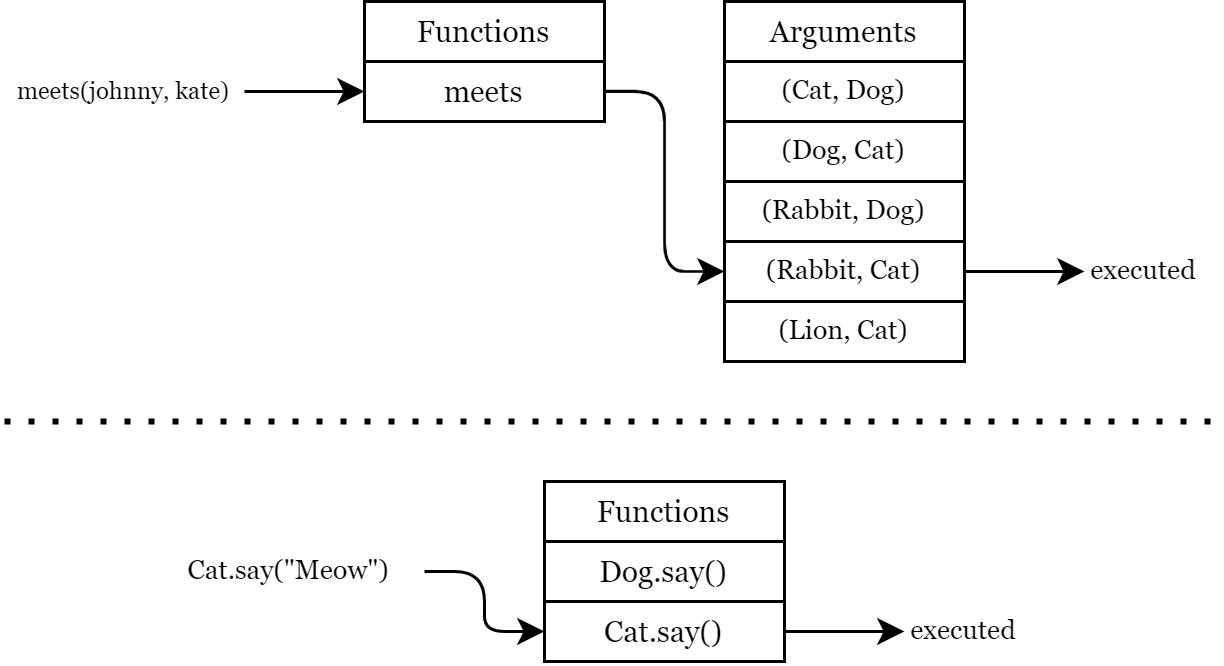
\includegraphics[width=1\textwidth]{multipleDispatch.png}
    \centering
    \caption{Multiple Dispatch (top) vs Single Dispatch (bottom) demonstrating that in the multiple dispatch paradigm, the executed function also depends on the type and order of its inputs} 
    \label{fig:multipleDispatch}
\end{figure}

\section{Type Heirarchy}
In Julia, all types are arranged in a tree-like structure and can be broadly classified into two categories, an Abstract
Type or a Concrete Type. Abstract types are the internal nodes of the type tree, having both parents and children, while
concrete types are the ``leaves'' of the tree, having parents but no children. Another notable difference between
abstract types and concrete types is that abstract types cannot be instantiated, they serve only as nodes in the type
graph. Shown in Figure \ref{fig:juliaTypeHeirarchy}, is the type hierarchy for the Integer type, abstract types are
highlighted in red, whereas concrete types are highlighted in blue. \hfill
\begin{figure}[t]
    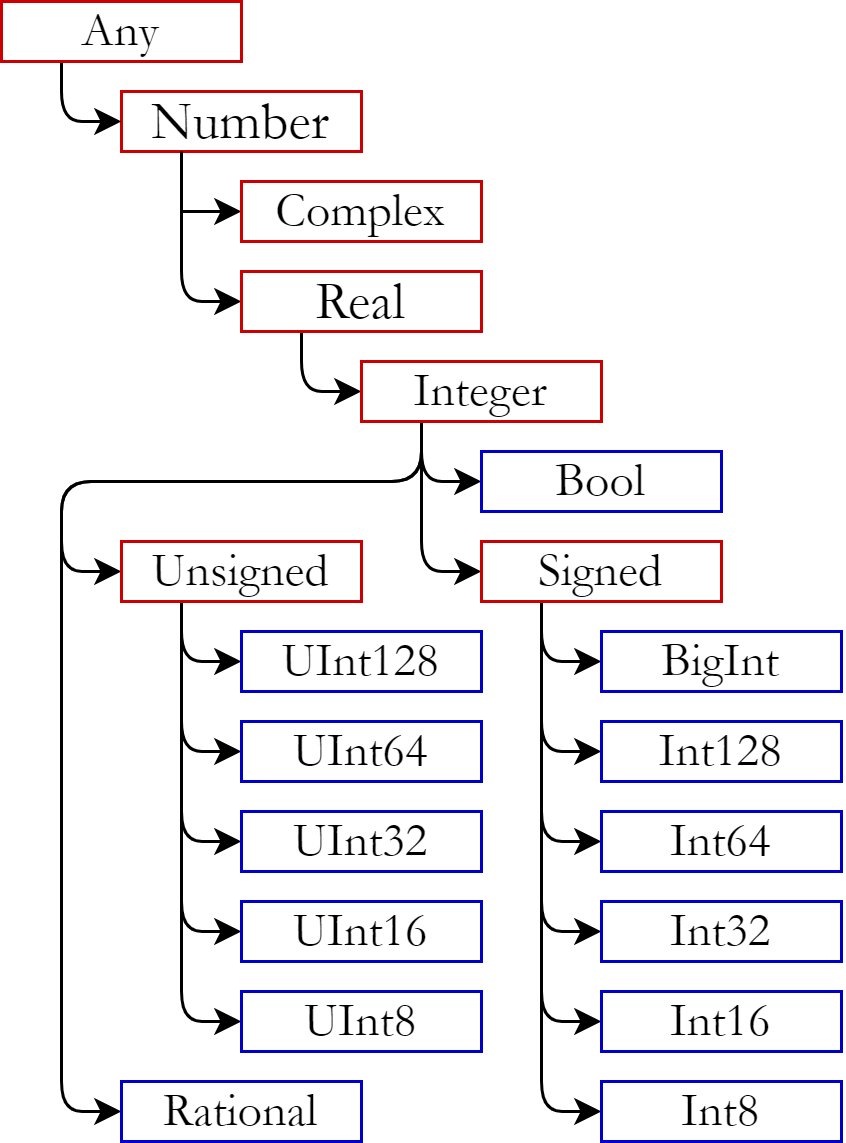
\includegraphics[width=0.45\textwidth]{juliaTypeTree.png}
    \centering
    \caption{Type hierarchy for the Integer Type} 
    \label{fig:juliaTypeHeirarchy}
\end{figure}
\FloatBarrier
The type hierarchy not only provides a way to logically organize types but also tightly integrates with the multiple
dispatch system mentioned before. It is this pairing that allows Julia to fulfill its promise of easy and powerful
extensibility. The following example helps illustrate this further.
\begin{lstlisting}[language=Julia]
# Defined in library A
abstract type Animal end

struct Cat <: Animal
    name::string
end

struct Dog <: Animal
    name::string
end

function encounters(petA::Animal, petB::Animal)
    verb = meets(petA, petB)
    println("$(petA.name) meets $(petB.name) and $(verb)")
end

meets(petA::Animal, petB::Animal) = "passes by."
meets(petA::Cat, petB::Dog) = "hisses"
meets(petA::Dog, petB::Cat) = "barks"

# Defined in library B
struct Rabbit <: Animal
    name::String
end

whiskers = Cat("Whiskers")
chomper = Rabbit("Chomper")
encounters(whiskers, chomper)
\end{lstlisting}
Library A defines a type hierarchy with Cat and Dog being a subtype of the abstract Animal type. The library then
implements a series of \lstinline[language=Julia]{meets} functions and an \lstinline[language=Julia]{ecounters}
function, similar to the example in the previous section. However, unlike the example before, there is a new
\lstinline[language=Julia]{meets} which accepts an argument of type Animal. Library B, importing library A, defines a
Rabbit type that is a subtype of the Animal abstract type and then calls the encounters function from library A. The
dispatch system cannot execute the \lstinline[language=Julia]{meets} function from lines 18, since
\lstinline[language=Julia]{chompers} is not of type Dog. Instead, it executes the \lstinline[language=Julia]{meets}
function on line 17, since both \lstinline[language=Julia]{whiskers} and \lstinline[language=Julia]{chompers} are valid
Animal types. This highlights an important interplay between the type hierarchy and the multiple dispatch system, in
that when dispatching, the Julia compiler will select the function that is most specific across all its input arguments.
The developer of library A need not worry about all the other possible Animal types, or what their fields may contain,
they can create a generic \lstinline[language=Julia]{meets} function that accepts any subtype of the Animal class and
will execute successfully provided the subtyped class contains the fields being accessed. Neither developer has to worry
about the completeness of the other's implementation, provided developer B follows the standards set by developer A,
they can develop an extension to library A and trust that the two libraries will be comparable.

\section{Parametric Polymorphism}
Parametric polymorphism refers to the programming paradigm where a function can be made generic to the input argument
type. At compilation time, the compiler can strongly type the function based on the types of the input arguments.
Consider the simple example of an \lstinline[language=Julia]{addtwo(x)} function.
\begin{lstlisting}[language=Julia]
function addTwo(x::T) where {T <: Real}
    return x + T(2)
end
\end{lstlisting}
Instead of specifying a concrete type for \lstinline[language=Julia]{x}, it is parametrized by the variable
\lstinline[language=Julia]{T} which has an abstract type restriction on it. This implies that
\lstinline[language=Julia]{T}, and by extension \lstinline[language=Julia]{x}, can by any type that is a subtype of the
Real abstract type. If parametric polymorphism was not a Julia feature, this function would have to be duplicated 16
times to account for the various concrete types that are a subtype of Real (see Figure \ref{fig:juliaTypeHeirarchy}).

\section{Type Stability}
\label{TypeStability}
Type Stability is a coding discipline that Julia recommends all code use. A function whose contained variables have a
consistent type for its lifetime is considered to be ``type stable'' or to have ``type stability''. Another way to think
about this, is that if the output type depends only on the input types, then the function is type stable. Consider the
following two functions: 
\begin{lstlisting}[language=Julia]
function unstable()
    x = 1
    for i = 1:10
        x /= rand()
    end
    return x
end

function stable()
    x = 1.0
    for i = 1:10
        x /= rand()
    end
    return x
end
\end{lstlisting}
Both functions have a variable, \lstinline[language=Julia]{x} which is divided 10 times by random floats and is returned
at the end of the function. However, based on the description above, the first function is considered to be ``Type
Unstable'' whereas the second function is considered to be ``Type Stable''. This is because in the first function the
type of \lstinline[language=Julia]{x} changes in the lifetime of the function (turns from Int64 to Float64). However in
the second function, the data type of \lstinline[language=Julia]{x} stays as a Float64 throughout the lifetime of the
function. The notion of type stability is important as it allows the Julia compiler to perform optimizations based on
the known data type of the variables at compile time. For type unstable functions, their unstable variables default to
type Any, ergo forgoing any optimizations. These optimizations are evident when benchmarking the functions above. This
was performed using the \lstinline[language=Julia]{@benchmark} macro from the BenchmarkTools module. Both functions were
run multiple times to ensure that only the compiled versions of the functions were executed rather than the interpreted
version. These benchmarks showed that on average the type unstable function ran 1.87x slower than the type stable
function (573.355~ns and 306.178~ns respectively).  

\section{Closure}
Closure in programming refers to the practice of calling a function A that returns a function B which has some
information about the variables contained in the scope of function A. Consider the following simple example:
\begin{lstlisting}[language=Julia]
function addX(x)
    scalar = x
    function calc_(a)
        return a + scalar
    end
end

add5 = addX(5)
add7 = addX(7)

add5(2)  # Will return 7
add7(10) # Will return 17
\end{lstlisting}
Defined above is a function called \lstinline[language=Julia]{addX} which accepts an input \lstinline[language=Julia]{x}
and assigns it to a variable \lstinline[language=Julia]{scalar}, before constructing and returning the function
\lstinline[language=Julia]{calc_}. This can be beneficial as it allows developers to create a family of functions that
are parametrized by their input variable.  It must be noted that the
captured variable, in the above case \lstinline[language=Julia]{scalar}, must never be reassigned, otherwise, the
compiler will not be able to infer the data types leading to type unstable code, and by extension all the negative
consequences mentioned in the previous section.

\section{Type Safety}
Type Safety refers to a program or language's ability to detect and discourage errors that arise from performing
operations on the wrong data type. For example in Julia, it is simple to add two numeric types, but performing the same
operation on two strings would yield an error, since the summation operator is not defined for two string types. This
offers some level of protection against illegal operations, but there are many cases where the type of the variables
agree with the operation being performed, but their semantic meaning disagrees. The example below will illustrate this
idea.
\begin{lstlisting}[language=Julia]
function calcSpeed(dist::Vector{T}, t::Vector{T}) where {T <: Real}
    return dist ./ t
end

#################################################### 
distance = rand(1, 100)
time = rand(1, 100)
calcSpeed(distance, time)   # Will compute the speed

#################################################### 
distance = rand(1, 100)
time = rand(ComplexF64,1, 100)

# Will throw an error since there is a type mismatch
calcSpeed(distance, time)  

#################################################### 
distance = rand(1, 100)
time = rand(1, 100)

# Will compute the wrong answer, but no error gets thrown
calcSpeed(time, distance) 
\end{lstlisting}
In the code block above \lstinline[language=Julia]{calcSpeed} accepts a vector of distance and time and returns the
associated speeds. Executing line 8, as expected returns the calculated speeds correctly. Executing line 12 will throw a
type error since ComplexF64 is not a subtype of Real. Line 22 however, will execute and return successfully even though
the wrong answer is returned, as the arguments were provided in the wrong positional order. This is because compilers
can only make inferences regarding the legality of a statement based solely on the concrete types of its arguments
rather than their semantic meaning in the context of the function being executed. However, the chance of variables being
incorrectly passed positionally can be negated by creating lightweight types that encode this semantic information in
their type name. In the above case, it would mean creating a ``distance'' type and a ``time'' type that act as wrappers
around a numerical concrete type. This way when line 22 is executed, instead of returning an incorrect answer, the
compiler will raise an error as the ``time'' and ``distance'' types were provided in the wrong order.